\documentclass[11pt,a4paper]{article}

\usepackage[utf8]{inputenc}
\usepackage[T1]{fontenc}
\usepackage{mathpazo}
\usepackage[scaled=0.92]{helvet}
\usepackage[margin=1in]{geometry}
\usepackage{graphicx}
\usepackage{amsmath,amssymb,amsfonts}
\usepackage{booktabs}
\usepackage{tabularx}
\usepackage{setspace}
\usepackage{titlesec}
\usepackage{fancyhdr}
\usepackage{float}
\usepackage{caption}
\usepackage{microtype}
\usepackage{tikz}
\usepackage{xcolor}
\usepackage[hidelinks]{hyperref}

\usetikzlibrary{shapes.geometric, arrows.meta, positioning, calc, matrix, fit, backgrounds}

\setstretch{1.15}
\setlength{\parindent}{0pt}
\setlength{\parskip}{0.8em}
\sloppy

\titleformat{\section}{\normalfont\large\bfseries\sffamily}{\thesection}{1em}{}
\titleformat{\subsection}{\normalfont\normalsize\bfseries\sffamily}{\thesubsection}{1em}{}
\titleformat{\subsubsection}{\normalfont\normalsize\itshape\sffamily}{\thesubsubsection}{1em}{}

\pagestyle{fancy}
\fancyhf{}
\fancyhead[L]{\small\sffamily Fondasi Tipe Data dalam Ilmu Komputer}
\fancyhead[R]{\small\sffamily\thepage}
\renewcommand{\headrulewidth}{0.4pt}

\captionsetup{font=small,labelfont=bf,labelsep=period}

\renewenvironment{abstract}
{\small
	\begin{center}\textbf{\sffamily Abstrak}\end{center}
	\begin{quote}}
	{\end{quote}}

\lstdefinestyle{code}{
	basicstyle=\ttfamily\small,
	frame=single,
	rulecolor=\color{black},
	breaklines=true,
	showstringspaces=false,
	columns=fullflexible,
	keepspaces=true,
	framesep=6pt,
	aboveskip=1em,
	belowskip=1em,
	xleftmargin=0pt
}

\lstdefinestyle{out}{
	basicstyle=\ttfamily\small,
	frame=tb,
	rulecolor=\color{black},
	breaklines=true,
	showstringspaces=false,
	columns=fullflexible,
	keepspaces=true,
	framesep=4pt,
	aboveskip=1em,
	belowskip=1em
}

\title{\vspace{-1.5cm}\textbf{\sffamily\LARGE Anatomi Tipe Data:\\ Dari Representasi Bit Hingga Sistem Tipe Tingkat Lanjut}}
\author{
	\textbf{Muhammad Riduwan Khafidi} \\
	\small Program Studi Teknik Rekayasa Perangkat Lunak \\
	\small Politeknik Negeri Batam \\
	\small \texttt{4342611034@students.polibatam.ac.id}
}
\date{\small\today}

\begin{document}
	
	\maketitle
	\thispagestyle{empty}
	
	\begin{abstract}
		Tipe data adalah fondasi fundamental dalam ilmu komputer yang mendefinisikan bagaimana nilai direpresentasikan, dioperasikan, dan dibatasi di dalam memori mesin. Makalah ini menyajikan kajian komprehensif mengenai tipologi data, mulai dari representasi biner tingkat mesin (machine types) hingga struktur abstrak tingkat tinggi seperti Dependent Types dan Refinement Types. Pembahasan mencakup definisi tipe data menurut literatur klasik, klasifikasi (atomik vs komposit), anatomi tipe primitif (Boolean, Numerik, String), tipe komposit (Array, Record), Abstract Data Types (ADT), hingga Algebraic Data Types yang populer di bahasa fungsional dan modern. Melalui sepuluh visualisasi diagram, makalah ini memetakan perjalanan data dari sekadar kumpulan bit hingga menjadi entitas yang bermakna dan aman secara logika. Makalah ini juga dilengkapi studi kasus perancangan sistem tipe, tabel kesalahan umum, dan lembar rujukan cepat.
	\end{abstract}
	
	\section{Pendahuluan}
	
	\subsection{Analogi Pembuka}
	
	Bayangkan sebuah gudang logistik yang sangat besar. Jika semua barang—mulai dari jarum jahit, televisi, hingga cairan kimia—dilempar begitu saja ke dalam satu ruangan tanpa rak atau kotak, gudang itu akan menjadi kekacauan. Barang-barang akan rusak, sulit ditemukan, dan berbahaya. Untuk mengelolanya, kita membutuhkan wadah yang spesifik: kotak kecil untuk jarum, peti kayu untuk televisi, dan drum anti-bocor untuk bahan kimia.
	
	Dalam dunia perangkat lunak, tipe data adalah sistem pengarsipan canggih tersebut. Komputer pada dasarnya bodoh; ia hanya mengenal tegangan listrik yang diterjemahkan menjadi angka 0 dan 1. Tipe data adalah instruksi kepada kompilator tentang bagaimana urutan 0 dan 1 tersebut harus ditafsirkan, seberapa besar ruang memori yang harus dicadangkan, dan operasi logika atau matematika apa yang legal untuk dilakukan.
	
	\subsection{Mengapa Topik Ini Penting}
	
	Pemilihan tipe data yang salah ibarat meminjamkan palu besi kepada tukang kaca. Program mungkin berjalan di permukaan, namun akan hancur berantakan saat menghadapi data dunia nyata. Memahami anatomi tipe data memisahkan antara penulis kode pemula dengan insinyur perangkat lunak yang mampu membangun sistem terdistribusi yang aman, efisien, dan bebas dari anomali.
	
	\subsection{Peta Pembahasan}
	
	Makalah ini disusun secara sistematis. Bagian kedua membedah definisi tipe data secara filosofis. Bagian ketiga mengklasifikasikan tipe data. Bagian keempat membahas tipe mesin dan primitif. Bagian kelima mengeksplorasi tipe komposit dan abstrak. Bagian keenam menyelami tipe data tingkat lanjut (Sistem Tipe). Bagian ketujuh menyajikan perbandingan, dilanjutkan dengan studi kasus, kesalahan umum, lembar rujukan cepat, dan kesimpulan.
	
	\section{Konsep dan Definisi Filosofis}
	
	Dalam literatur ilmu komputer, definisi "tipe" seringkali bersifat implisit. Parnas, Shore, dan Weiss (1976) mengidentifikasi lima cara mendefinisikan tipe data:
	
	Pertama, definisi \textbf{Sintaksis}, di mana tipe hanyalah label murni yang menempel pada variabel saat dideklarasikan. Kedua, definisi \textbf{Representasi}, di mana tipe didefinisikan berdasarkan komposisi tipe primitif di tingkat mesin. Ketiga, \textbf{Representasi dan Perilaku}, yang menambahkan sekumpulan operator (fungsi) yang memanipulasi representasi tersebut.
	
	Keempat, definisi \textbf{Ruang Nilai} (\textit{Value Space}), di mana tipe adalah himpunan nilai yang mungkin dimiliki oleh sebuah variabel. Kelima, \textbf{Ruang Nilai dan Perilaku}, yang menggabungkan himpunan nilai dengan himpunan fungsi yang dapat diterapkan padanya. Pendekatan ruang nilai dan perilaku inilah yang paling dekat dengan pemodelan \textit{Object-Oriented Programming} (OOP) modern.
	
	Perbedaan semantik juga sangat krusial. Tipe \texttt{int} di Python merepresentasikan bilangan bulat dengan presisi arbitrer (sebesar memori yang tersedia). Namun, tipe \texttt{int} di Java adalah bilangan bulat 32-bit yang kaku (berkisar $-2.147.483.648$ hingga $2.147.483.647$). Jika melebihi batas, Java akan mengalami \textit{integer overflow} (nilai berputar kembali ke negatif). Di Rust, tipe 32-bit ini dinamakan \texttt{i32}, dan alih-alih berputar, program akan sengaja dihentikan (\textit{panic}) saat mode \textit{debug} untuk mencegah \textit{bug} logika.
	
	\section{Klasifikasi Tipe Data}
	
	Tipe data dapat dikategorikan berdasarkan beberapa faktor. Berdasarkan asalnya, ada \textbf{Tipe Primitif} (bawaan bahasa) dan \textbf{Tipe Buatan Pengguna} (\textit{User-defined}). Berdasarkan strukturnya, ada \textbf{Tipe Atomik} (satu item yang tak terpecahkan, seperti integer) dan \textbf{Tipe Komposit} (kumpulan item yang bisa diakses terpisah, seperti array). 
	
	Selain itu, ada \textbf{Tipe Dasar} (\textit{Basic}) yang didefinisikan secara aksiomatik (misal: integer dalam matematika), dan \textbf{Tipe Turunan} (\textit{Generated/Derived}) yang dibangun dari tipe lain (misal: array dari integer). 
	
	\begin{figure}[H]
		\centering
		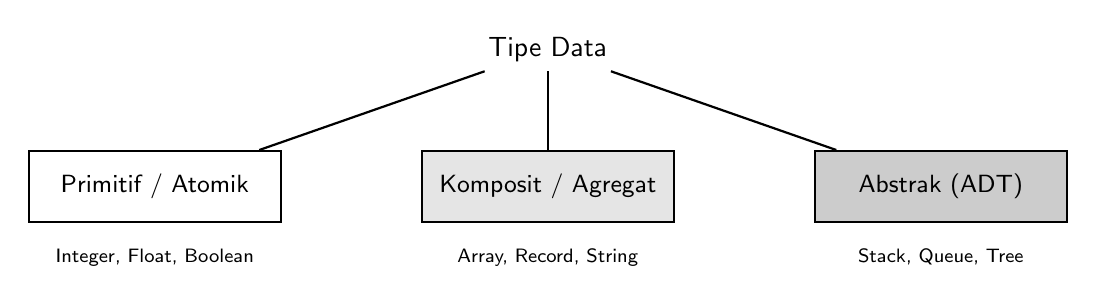
\begin{tikzpicture}[
				node distance=0.5cm and 0.8cm,
				cat/.style={rectangle, draw=black, thick, minimum width=3.2cm, minimum height=0.9cm, align=center, font=\sffamily\small},
				line/.style={draw, thick}
			]
			\node[font=\sffamily] (root) at (0, 1.5) {Tipe Data};
			\node[cat, fill=white, below left=1cm and 2.5cm of root] (prim) {Primitif / Atomik};
			\node[cat, fill=black!10, below=1cm of root] (comp) {Komposit / Agregat};
			\node[cat, fill=black!20, below right=1cm and 2.5cm of root] (abs) {Abstrak (ADT)};
			
			\draw[line] (root) -- (prim);
			\draw[line] (root) -- (comp);
			\draw[line] (root) -- (abs);
			
			\node[font=\scriptsize\sffamily, below=0.2cm of prim] {Integer, Float, Boolean};
			\node[font=\scriptsize\sffamily, below=0.2cm of comp] {Array, Record, String};
			\node[font=\scriptsize\sffamily, below=0.2cm of abs] {Stack, Queue, Tree};
		\end{tikzpicture}
		\caption{Klasifikasi hierarkis tipe data.}
		\label{fig:hierarchy-types}
	\end{figure}
	
	\section{Tipe Mesin dan Primitif}
	
	Di tingkat terendah, semua data direpresentasikan sebagai \textit{bit} (0 dan 1). Unit terkecil yang dapat dialamatkan adalah \textit{byte} (8 bit). Unit yang diproses oleh instruksi mesin disebut \textit{word} (umumnya 32 atau 64 bit). 
	
	Tipe mesin memberikan kendali presisi atas perangkat keras, namun mengorbankan portabilitas. Bahasa tingkat tinggi seperti C menyediakan tipe Boolean, integer, dan float, namun representasi bit pastinya ditentukan oleh implementasi kompilator. Hanya tipe \texttt{char} di C yang dijamin berukuran tepat satu byte.
	
	\subsection{Tipe Boolean}
	Tipe Boolean hanya memiliki dua nilai: Benar (\textit{true}) dan Salah (\textit{false}). Secara logis, ini hanya butuh 1 bit. Namun, karena arsitektur CPU modern membaca data dalam blok memori, Boolean seringkali tetap memakan 1 byte penuh. Banyak bahasa (seperti C versi lama) tidak memiliki Boolean eksplisit, melainkan menggunakan integer dengan konvensi 0 untuk Salah dan bukan-nol untuk Benar.
	
	\subsection{Tipe Numerik}
	Integer adalah tipe dasar bilangan bulat. Jika tipe 32-bit dipaksakan pada platform 16-bit, kompilator akan memecahnya menjadi dua integer 16-bit. 
	
	Untuk bilangan pecahan, terdapat \textbf{Floating-point} (IEEE 754) yang menyimpan angka dalam notasi ilmiah biner ($a \times 2^b$). Tipe ini memiliki jangkauan luas, namun rentan terhadap galat pembulatan (misalnya $0.1 + 0.2 \neq 0.3$ secara eksak). Sebaliknya, \textbf{Fixed-point} menyimpan angka desimal dengan mengalikannya menjadi integer (misal 12.34 disimpan sebagai 1234), sehingga presisi eksak terjaga, sangat cocok untuk aplikasi finansial.
	
	Untuk angka yang sangat besar, tersedia \textbf{Bignum} (\textit{Arbitrary-precision arithmetic}), yang batasannya hanya memori komputer, meskipun operasi matematikanya jauh lebih lambat.
	
	\begin{figure}[H]
		\centering
		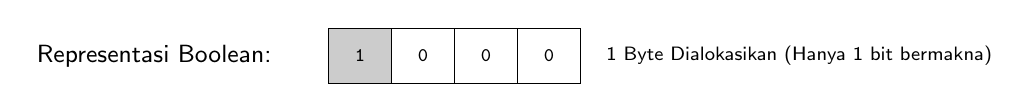
\begin{tikzpicture}[
				cell/.style={rectangle, draw=black, minimum width=0.8cm, minimum height=0.7cm, font=\ttfamily\scriptsize, align=center},
				lbl/.style={font=\sffamily\small}
			]
			\node[lbl, anchor=east] at (-1, 0) {Representasi Boolean:};
			\node[cell, fill=black!20] (a1) at (0, 0) {1};
			\node[cell, fill=white]    (a2) at (0.8, 0) {0};
			\node[cell, fill=white]    (a3) at (1.6, 0) {0};
			\node[cell, fill=white]    (a4) at (2.4, 0) {0};
			\node[font=\scriptsize\sffamily, right=0.2cm of a4] {1 Byte Dialokasikan (Hanya 1 bit bermakna)};
		\end{tikzpicture}
		\caption{Representasi memori tipe Boolean.}
		\label{fig:boolean}
	\end{figure}
	
	\section{Tipe Teks, Komposit, dan Abstrak}
	
	\subsection{String dan Karakter}
	String adalah urutan karakter yang diambil dari set karakter seperti ASCII atau Unicode (UTF-8). Tipe string dapat berupa panjang tetap (\textit{fixed-length}) yang selalu memakan memori sama, atau panjang variabel (\textit{variable-length}) yang menyesuaikan panjang teks. String numerik seperti \texttt{"1234"} secara semantik berbeda dengan integer \texttt{1234}, meskipun beberapa bahasa memfasilitasi konversi otomatis.
	
	\subsection{Union Types}
	Tipe Union mendefinisikan bahwa suatu variabel dapat menampung salah satu dari beberapa subtipe yang diizinkan (misal: \texttt{float} ATAU \texttt{long integer}). Berbeda dengan \textit{Record} yang menampung keduanya sekaligus, Union hanya menyimpan satu nilai pada satu waktu. \textit{Tagged Union} menambahkan field penanda tipe untuk keamanan ekstrak data.
	
	\subsection{Algebraic Data Types (ADT)}
	ADT adalah gabungan dari \textit{Sum Type} (tipe penjumlahan, "ATAU") dan \textit{Product Type} (tipe perkalian, "DAN"). Nilai ADT terdiri dari tag konstruktor dan field nilai. Contoh klasiknya adalah tipe \texttt{Option} (Haskell: \texttt{data Maybe a = Nothing | Just a}), yang digunakan untuk menangani nilai kosong secara aman tanpa \textit{null pointer exception}.
	
	\begin{figure}[H]
		\centering
		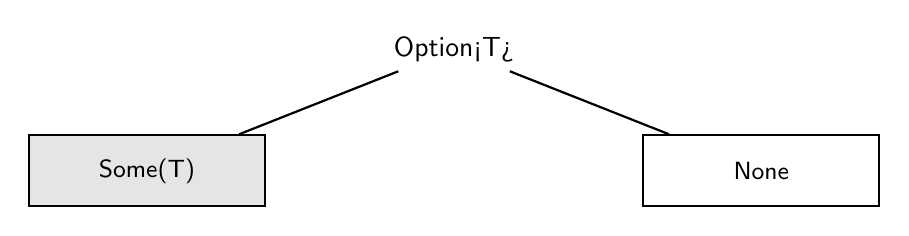
\begin{tikzpicture}[
				node distance=0.5cm and 1cm,
				cat/.style={rectangle, draw=black, thick, minimum width=3cm, minimum height=0.9cm, align=center, font=\sffamily\small},
				line/.style={draw, thick}
			]
			\node[font=\sffamily] (root) at (0, 1) {Option<T>};
			\node[cat, fill=black!10, below left=0.8cm and 1.5cm of root] (some) {Some(T)};
			\node[cat, fill=white, below right=0.8cm and 1.5cm of root] (none) {None};
			
			\draw[line] (root) -- (some);
			\draw[line] (root) -- (none);
		\end{tikzpicture}
		\caption{Sum Type pada tipe Option (Mungkin berisi nilai, mungkin kosong).}
		\label{fig:sumtype}
	\end{figure}
	
	\subsection{Struktur Data dan Abstract Data Types (ADT)}
	Struktur data adalah tipe komposit yang digunakan untuk menyimpan dan mengambil data. Contohnya adalah \textbf{Array} (akses acak via indeks), \textbf{Record} (kumpulan field bernama), \textbf{Linked List} (node yang saling terhubung), dan \textbf{Binary Tree} (pohon pencarian cepat).
	
	Di atas struktur data, terdapat \textit{Abstract Data Type} (ADT). ADT tidak mendefinisikan representasi konkret, melainkan hanya spesifikasi operasi (seperti \texttt{push} dan \texttt{pop} pada Stack). Implementasi di baliknya bisa menggunakan Array atau Linked List, selama aturan LIFO (Last-In-First-Out) terpenuhi.
	
	\section{Tipe Tingkat Lanjut (Sistem Tipe)}
	
	Ilmu komputer teoretis mengembangkan sistem tipe yang jauh lebih canggih untuk menjamin kebenaran program.
	
	\subsection{Pointers dan References}
	Pointer adalah tipe data yang nilainya merujuk pada alamat memori nilai lain. Ini adalah bentuk referensi primitif. Jika pointer menunjuk ke alamat memori yang tidak valid (misal: sudah dihapus), upaya untuk melakukan \textit{dereference} akan menyebabkan program \textit{crash}. Oleh karena itu, sistem tipe modern memisahkan pointer dari integer biasa, meskipun representasi bit-nya sama.
	
	\subsection{Function Types}
	Dalam bahasa fungsional (dan JavaScript), fungsi diperlakukan sebagai tipe data kelas satu (\textit{first-class citizen}). Fungsi dapat disimpan dalam variabel dan dioperasikan. Sistem tipe mendefinisikan tipe fungsi berdasarkan argumen dan nilai kembaliannya, misalnya \texttt{Int -> Bool}.
	
	\subsection{Type Constructors}
	Konstruktor tipe adalah operator yang membangun tipe baru dari tipe lama. Contohnya adalah \texttt{List<T>} yang membangun tipe List dari tipe T, atau \texttt{Product} yang menggabungkan dua tipe.
	
	\subsection{Quantified Types}
	Berdasarkan logika predikat, tipe dapat dikuantifikasi. \textit{Universal Quantification} ($\forall x. f(x)$) berarti nilai tersebut bertipe $f(x)$ untuk semua tipe $x$. \textit{Existential Quantification} ($\exists x. f(x)$) berarti ada tipe $x$ tertentu yang memenuhi.
	
	\subsection{Refinement Types}
	Tipe yang dilengkapi dengan predikat logika. Misalnya, tipe bilangan asli yang lebih besar dari 5 ditulis sebagai $\{n \in \mathbb{N} \mid n > 5\}$. Ini memungkinkan kompilator menolak nilai yang tidak memenuhi syarat matematis sebelum program berjalan.
	
	\begin{figure}[H]
		\centering
		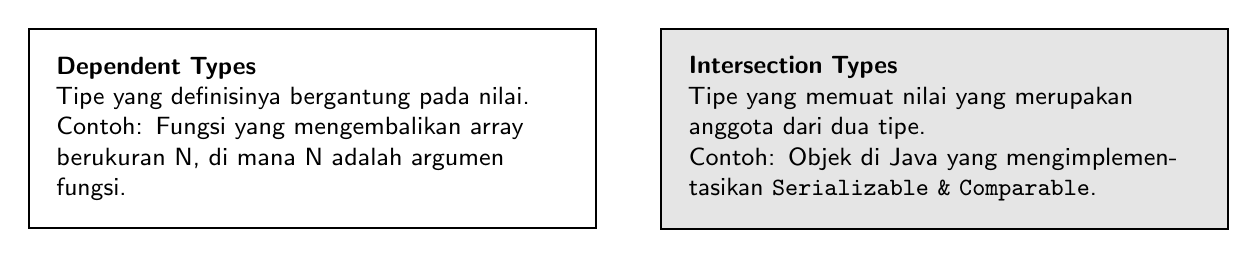
\begin{tikzpicture}[
				box/.style={rectangle, draw=black, thick, text width=6.5cm, align=left, font=\sffamily\small, inner sep=10pt}
			]
			\node[box, fill=white] (a) {
				\textbf{Dependent Types} \\
				Tipe yang definisinya bergantung pada nilai. \\
				Contoh: Fungsi yang mengembalikan array berukuran N, di mana N adalah argumen fungsi.
			};
			\node[box, fill=black!10, right=0.8cm of a] (b) {
				\textbf{Intersection Types} \\
				Tipe yang memuat nilai yang merupakan anggota dari dua tipe. \\
				Contoh: Objek di Java yang mengimplementasikan \texttt{Serializable \& Comparable}.
			};
		\end{tikzpicture}
		\caption{Perbandingan Dependent Types dan Intersection Types.}
		\label{fig:advanced}
	\end{figure}
	
	\section{Perbandingan}
	
	\begin{table}[H]
		\centering
		\caption{Ringkasan perbandingan seluruh kategori tipe data.}
		\label{tab:summary}
		\footnotesize
		\begin{tabularx}{\textwidth}{l X X}
			\toprule
			Kategori & Contoh & Karakteristik Utama \\
			\midrule
			Tipe Mesin & Byte, Word & Kontrol hardware langsung, tidak portabel \\
			Primitif & Integer, Boolean, Float & Atomik, batas memori jelas \\
			Teks & String, Char & Berbasis encoding, array karakter \\
			Komposit & Array, Record & Mengelompokkan data, akses per indeks/field \\
			Abstrak (ADT) & Stack, Queue & Spesifikasi operasi, menyembunyikan implementasi \\
			Aljabar (ADT) & Option, Result & Sum dari Product, aman dari null \\
			Referensi & Pointer, Reference & Menunjuk alamat memori, rawan crash \\
			Fungsi & Function Object & Fungsi sebagai nilai variabel \\
			Kuantifikasi & forall, exists & Logika predikat dalam tipe \\
			Refinement & $\{n \mid n > 5\}$ & Tipe dengan batasan predikat matematis \\
			Dependent & Dependent Pair & Tipe bergantung pada nilai spesifik \\
			Intersection & \texttt{A \& B} & Menggabungkan sifat dua tipe \\
			\bottomrule
		\end{tabularx}
	\end{table}
	
	\section{Studi Kasus: Perancangan Sistem Tipe E-Commerce}
	
	\subsection{Langkah 1: Identifikasi Kebutuhan}
	Kita akan merancang tipe data untuk produk e-commerce yang memiliki nama, harga, stok, dan status (tersedia/habis).
	
	\subsection{Langkah 2: Tipe String untuk Nama}
	Nama produk menggunakan tipe \texttt{String} karena panjangnya dinamis.
	
	\subsection{Langkah 3: Tipe Numerik untuk Harga}
	Harga tidak boleh menggunakan \texttt{Float} karena akan merusak perhitungan uang. Kita gunakan \texttt{Decimal} atau \texttt{Integer} (dalam satuan sen).
	
	\subsection{Langkah 4: Tipe Integer untuk Stok}
	Stok barang menggunakan \texttt{u32} (unsigned 32-bit integer) karena tidak mungkin bernilai negatif.
	
	\subsection{Langkah 5: Enum untuk Status}
	Status produk adalah Enum (tipe enumerasi): \texttt{Tersedia} atau \texttt{Habis}.
	
	\subsection{Langkah 6: Record untuk Produk}
	Semua field di atas digabungkan menjadi satu tipe \texttt{Record} (Struct).
	
	\subsection{Langkah 7: Penanganan Opsional}
	Apa yang terjadi jika produk memiliki diskon? Kita gunakan \texttt{Option<Diskon>} di mana jika tidak ada diskon, nilainya \texttt{None}.
	
	\subsection{Langkah 8: Implementasi Tipe}
	
	\begin{lstlisting}[style=code]
struct Produk {
    id: u64,
    nama: String,
    harga: Decimal,
    stok: u32,
    status: StatusProduk,
    diskon: Option<Decimal>,
}
	
enum StatusProduk {
    Tersedia,
    Habis,
}
	\end{lstlisting}
	
	\section{Kesalahan Umum dan Cara Menghindarinya}
	
	\begin{table}[H]
		\centering
		\caption{Kesalahan umum terkait tipe data.}
		\label{tab:mistakes}
		\footnotesize
		\begin{tabularx}{\textwidth}{l X X}
			\toprule
			Kesalahan & Akibat & Perbaikan \\
			\midrule
			\textit{Integer overflow} & Nilai berputar negatif secara acak & Gunakan Bignum atau tipe 64-bit \\
			\textit{Float} untuk uang & Galat akumulatif pada transaksi & Gunakan Decimal atau Fixed-point \\
			\textit{Null Pointer} & Program \textit{crash} & Gunakan Option / Nullable Type \\
			Salah encoding teks & Teks menjadi karakter aneh (Mojibake) & Standarkan pada UTF-8 \\
			\textit{Type casting} paksa & Kehilangan data (misal float ke int) & Gunakan konversi aman atau cek rentang \\
			Mengabaikan Signed/Unsigned & \textit{Bug} saat nilai dimasukkan negatif & Gunakan \textit{signed} jika perlu nilai minus \\
			\textit{Pointer arithmetic} liar & Akses memori ilegal (Segfault) & Gunakan Reference / Smart Pointer \\
			Mengabaikan tipe fungsi & Callback error & Definisikan tipe fungsi secara eksplisit \\
			\bottomrule
		\end{tabularx}
	\end{table}
	
	\section{Lembar Rujukan Cepat}
	
	\begin{table}[H]
		\centering
		\caption{Rujukan cepat pemilihan tipe data.}
		\label{tab:cheat}
		\footnotesize
		\begin{tabularx}{\textwidth}{l X}
			\toprule
			Kebutuhan & Tipe Data atau Representasi \\
			\midrule
			Bilangan bulat umum & \texttt{int} (32-bit) atau \texttt{i32} \\
			Bilangan bulat besar & \texttt{i64} atau \texttt{BigInt} \\
			Bilangan desimal ilmiah & \texttt{float} (32-bit) atau \texttt{double} (64-bit) \\
			Mata uang / Finansial & \texttt{Decimal} atau \texttt{Fixed-Point} \\
			Teks dinamis & \texttt{String} atau \texttt{VARCHAR} \\
			Teks statis & \texttt{CHAR(n)} \\
			Nilai Benar/Salah & \texttt{Boolean} \\
			Data kosong (mungkin ada) & \texttt{Option<T>} atau \texttt{Nullable} \\
			Kumpulan data sejenis & \texttt{Array} atau \texttt{Vector} \\
			Data berpasangan & \texttt{Struct} atau \texttt{Tuple} \\
			Kumpulan status tetap & \texttt{Enum} \\
			Fungsi sebagai argumen & \texttt{Function Type} \\
			Referensi memori aman & \texttt{\&T} atau \texttt{Reference} \\
			Alamat memori mentah & \texttt{Pointer} (Hindari jika bisa) \\
			Pembatasan nilai logika & \texttt{Refinement Type} \\
			\bottomrule
		\end{tabularx}
	\end{table}
	
	\section{Kesimpulan}
	
	Tipe data bukan sekadar sintaks deklarasi, melainkan pilar utama dalam menjamin keamanan dan kebenaran perangkat lunak. Tiga prinsip penutup:
	
	\begin{enumerate}
		\item Tipe adalah Kontrak. Pemilihan tipe data adalah perjanjian antara pengembang dan mesin tentang bagaimana memori dikelola dan operasi apa yang legal.
		\item Representasi Menentukan Batasan. Memahami bahwa \texttt{Float} memiliki galat atau \texttt{Integer} bisa meluap (overflow) adalah kunci untuk menulis algoritma yang tangguh.
		\item Abstraksi Memberi Skalabilitas. Dari tipe primitif hingga \textit{Dependent Types}, tipe data memungkinkan manusia memodelkan logika dunia nyata yang paling kompleks ke dalam sistem yang dapat dieksekusi oleh mesin secara aman.
	\end{enumerate}
	
	\newpage
	\section*{Referensi}
	\addcontentsline{toc}{section}{Referensi}
	
	\begin{thebibliography}{99}
		
		\bibitem{parnas}
		Parnas, D. L., Shore, J. E., \& Weiss, D. (1976).
		Abstract types defined as classes of variables.
		\textit{Proceedings of the 1976 conference on Data: Abstraction, definition and structure}, 149--154.
		\texttt{https://doi.org/10.1145/800237.807133}
		
		\bibitem{silberschatz}
		Silberschatz, A., Korth, H. F., \& Sudarshan, S. (2019).
		\textit{Database System Concepts} (7th ed.).
		McGraw-Hill Education.
		
		\bibitem{ieee754}
		IEEE. (2019).
		\textit{IEEE Standard for Floating-Point Arithmetic
			(IEEE 754-2019)}.
		Institute of Electrical and Electronics Engineers.
		
		\bibitem{klabnik}
		Klabnik, S., \& Nichols, C. (2019).
		\textit{The Rust Programming Language}.
		No Starch Press.
		
		\bibitem{brookshear}
		Brookshear, J. G. (2019).
		\textit{Computer Science: An Overview} (13th ed.).
		Pearson.
		
		\bibitem{cardelli}
		Cardelli, L., \& Wegner, P. (1985).
		On Understanding Types, Data Abstraction, and Polymorphism.
		\textit{ACM Computing Surveys}, 17(4), 471--523.
		\texttt{https://doi.org/10.1145/6041.6042}
		
		\bibitem{wikipedia-datatype}
		Wikipedia Contributors. (2026, September 16).
		\textit{Data type}.
		Wikipedia, The Free Encyclopedia.
		\texttt{https://en.wikipedia.org/wiki/Data\_type}
		
	\end{thebibliography}
	
\end{document}